\documentclass{sig-alternate}
\usepackage{url}
\usepackage{color}
\usepackage{algorithm}
\usepackage{algpseudocode}
\usepackage{syntax}
\usepackage{caption}
\usepackage[final]{listings}
\toappear{}

\newcommand{\da}{\emph{Dragon Architect}}
\newcommand{\todo}[1]{{\color{red} TODO: #1}}

\newenvironment{BNF}
  {\captionsetup{type=lstlisting}}
  {}

\begin{document}
\title{Optimizing in a Novice Programming Environment}
\author{Eric Butler \and Aaron Bauer}
\maketitle{}

\begin{abstract}
\da{}, our programming system for novices, encounters performance problems when handling large user programs. This is primarily due to a slider bar that allows the user to scrub throughout a program's execution, for which we inefficiently precompute all program states. To improve performance on large programs we implemented and evaluated two dynamic optmizations. The first precomputes as few states as possible, and instead caches results from procedure calls and loop bodies as \emph{deltas} on the world state. The second precomputes a fixed number of states, and uses them as checkpoints to compute intermediate states quickly. Our evaluation shows both are \todo{WHATEVER IT SHOWS}.
\end{abstract}

\section{Introduction}

For the past year, we have been developing \da, a programming system for novices, for the purpose of exploring research questions in computer science pedagogy and language usability for novices. Core to the design of our tool is to provide both a \emph{low floor} and \emph{high ceiling}, which is important for both supporting a wide range of skill levels, and engaging students over an extended progression. Part of our vision for students' progression through \da{} is tackling programs of increasing size and sophistication. The system also includes several debugging tools, and we are interested in studying when and how various debugging tools are beneficial to novices. 

For example, our system supports debugging tool that allows users to move the program execution state forward and backward in time by dragging a slider bar. Thus, the language simulator needs to be able to quickly jump to different points of execution. In the presence of larger programs, however, the na\"{i}ve implementation of this slider bar, storing an array of all program states, quickly runs into scalability issues. Optimization of our runtime became necessary to support large programs efficiently. 

Fortunately, ample optimization opportunities exist. The design of \da{}'s language is intentionally very simple, to increase accessibility for novices. As a consequence, large programs are both very repetitive and deterministic. To try to improve performance on larger programs, we investigated and created two dynamic optimization techniques. One aggressively caches and reuses results for procedure calls and loop bodies, and the other computes a small number of \emph{checkpoints} instead of every state, resimulating from the nearest checkpoint when necessary. Our evaluation shows \todo{SOMEHTING PROBABLY?}

\section{Related Work}
There has been a great deal of previous work on programming environments for novices, including prominent examples like Scratch ~\cite{resnick2009scratch} and Alice~\cite{cooper2000alice}. We are not aware, however, of any existing work on optmizations in this kind of environment. 

There is a long history of work on static analysis (e.g.,~\cite{cousot1977abstract}), but given that our programs take no input and are deterministic, performing dynamic analysis is clearly preferable. The many techniques developed for just-in-time (JIT) compilation~\cite{aycock2003brief} are more appropriate, but are intend for far more complex programming models than the simple one in \da.

The concept behind our time slider bar is not novel, as previous work as has dealt with navigating program execution as a timeline for both novices~\cite{ko2004designing} and professional web development~\cite{burg2013interactive}. Our environment differs considerably from those in previous work, however, so we have designed optimizations specifically suited to the opportunities and constraints in \da.

\section{Background}

We first discuss technical details of the language and runtime environment used in \da. To summarize, execution in \da{} consists of running a simple imperative language to compute a list of commands for the dragon in the 3d world, and this list of commands is applied to compute a new world state. An example program and resulting world state is shown in Figure~\ref{fig:full-program}. The summary of the grammar is given by Listing~\ref{lst:grammar}, though there is actually both a textual concrete representation (shown the in the appendix) and a visual block-based representation.

\begin{BNF}
\caption{\da{} grammar}
\label{lst:grammar}
\begin{grammar}
<expr> ::= <ident> | <integer>

<arglist> ::= <expr> `,' <arglist> | <expr>

<args> ::= `(' `)' | `(' <arglist> `)'

<paramlist> ::= <ident> `,' <paramlist> | <ident>

<params> ::= `(' `)' | `(' <paramlist> `)'

<statement> ::= <ident> <args>
\alt `repeat' <expr> `times' <block>
\alt `command' <ident> <args>
\alt `define' <ident> <params> <block>

<block> ::= <statement> <block> | <statement>
\end{grammar}
\end{BNF}

\begin{figure*}[t!]
  \centering
  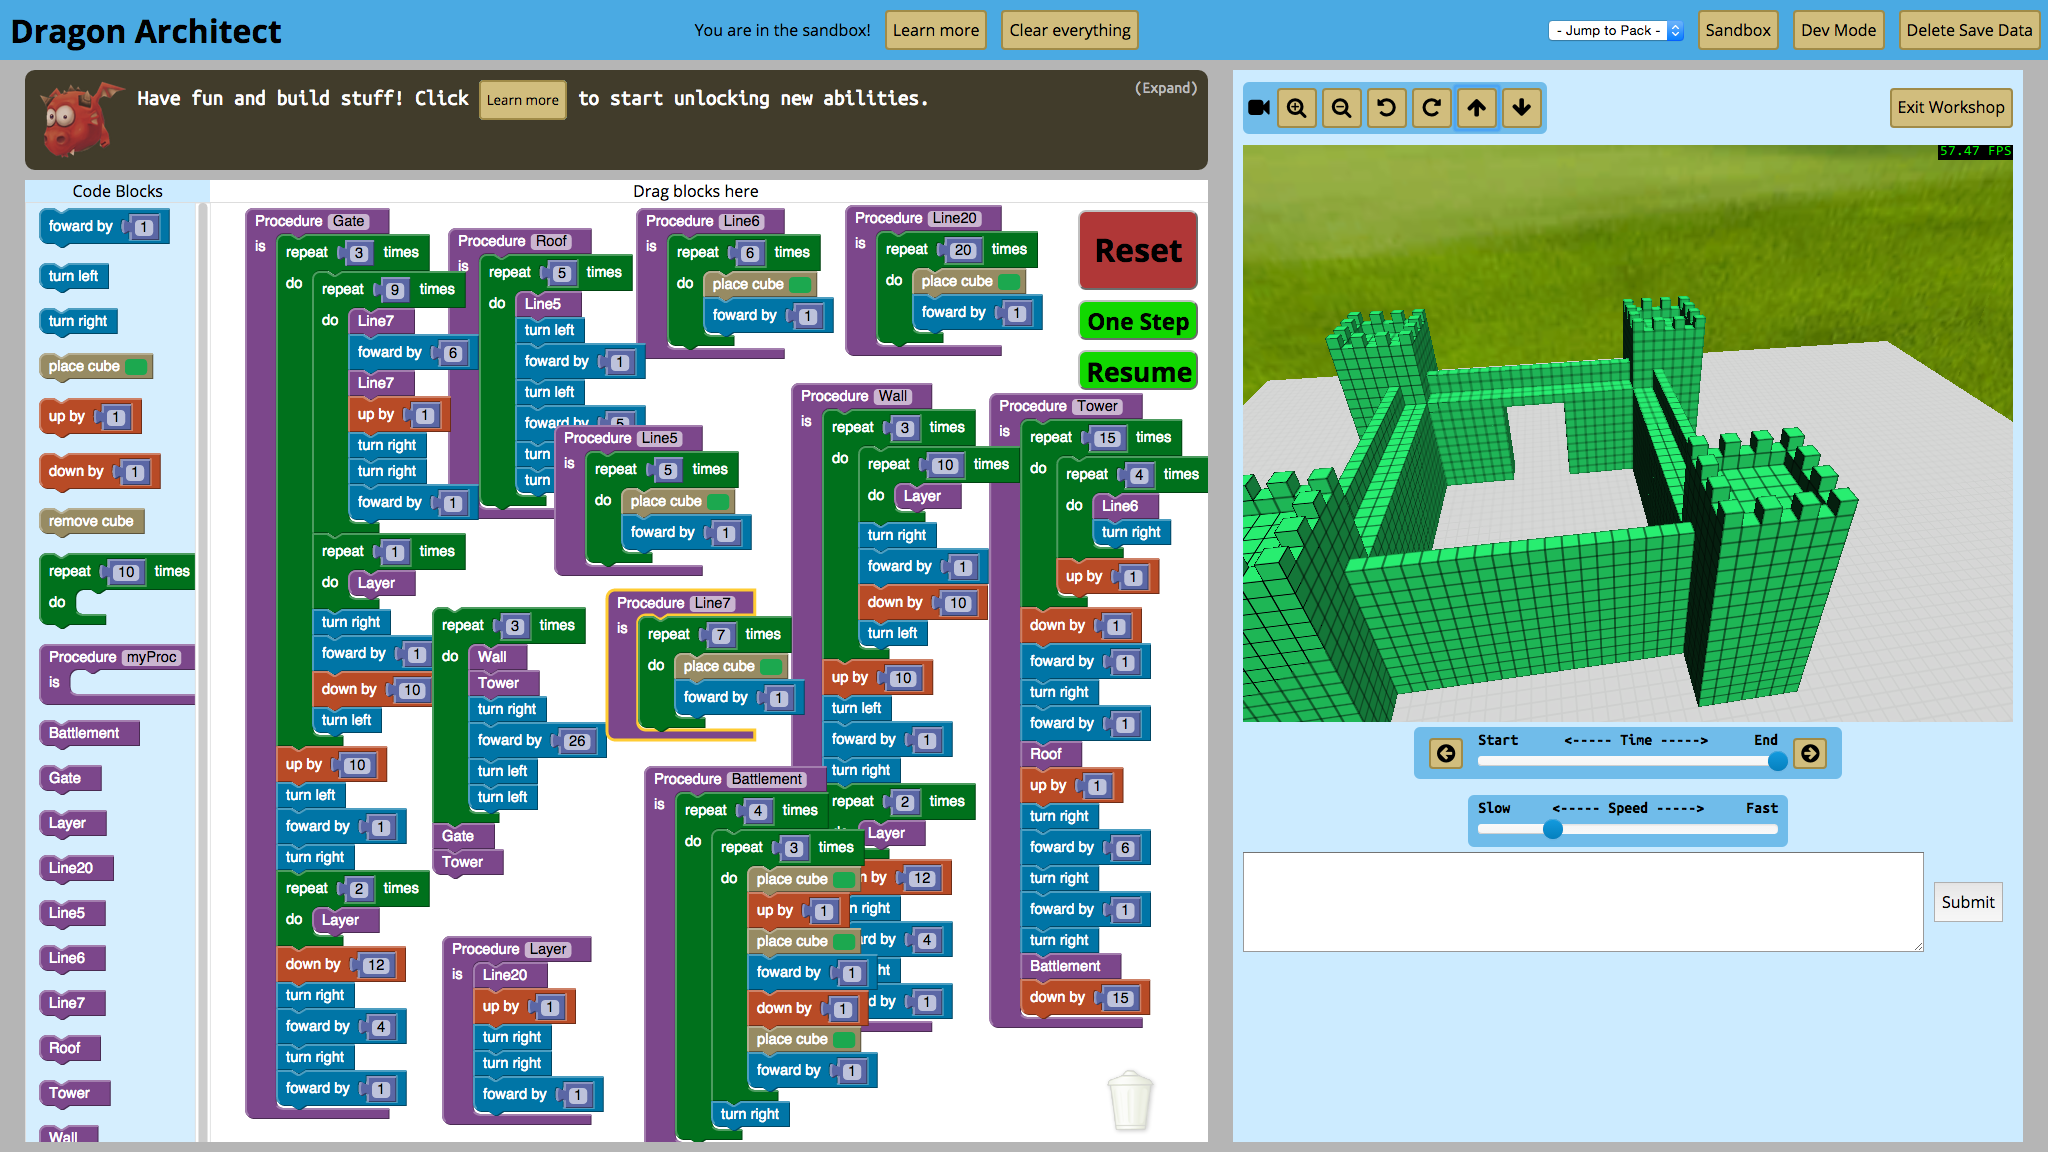
\includegraphics[width=0.9\textwidth]{images/full-castle}
  \caption{A screenshot of the \da{} application with an example program that builds a castle. The student edits the code on the left, and the result is displayed on the right. A textual representation of an equivalent program is given in the appendix.}
  \label{fig:full-program}
\end{figure*}

We elide a fully formal description of \da's language semantics and instead briefly describe how programs behave. The \texttt{command} statements describe operations for the dragon to perform in the 3d world. Because our language currently does not have any conditionals, this list of commands does not depend on the world state, or even what the semantics of the world are. Thus, program execution can be thought of as two phases, one in which the list of commands is computed, and another in which the list of commands is applied to the world state to compute the final world state. This is summarized in Figure~\ref{fig:phases}.

\begin{figure*}[ht!]
  \centering
  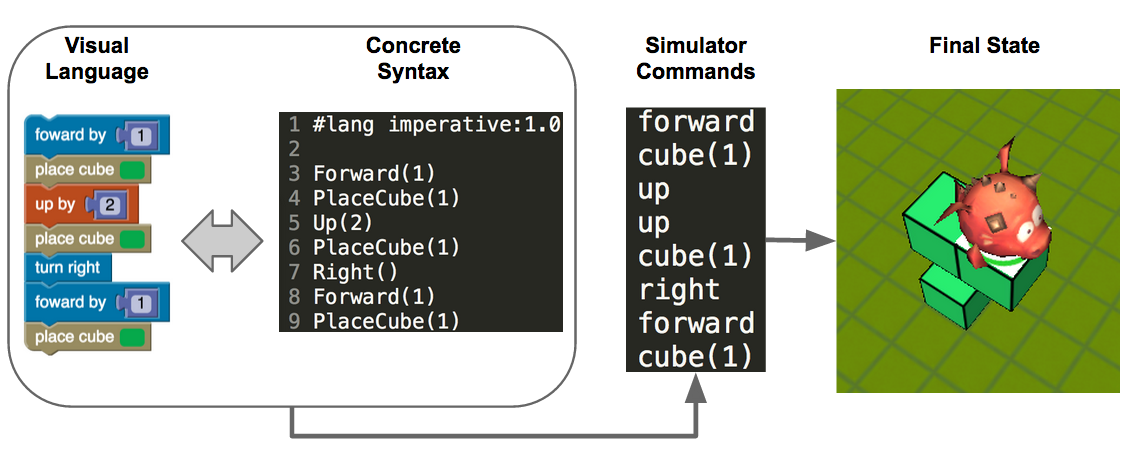
\includegraphics[width=0.9\textwidth]{images/phases}
  \caption{A diagram of the phases of program execution in \da{}. The first phase converts the concrete syntax, which can be either visual drag-and-drop or text-based, into a sequence of commands. The visual and text versions of the language have a one-to-one correspondence. The second phase simulates these commands to produce a resulting world state (i.e., dragon position, dragon direction, and placed cubes).}
  \label{fig:phases}
\end{figure*}

The other statements in \da{} behave similarly to constructs in most other imperative programming languages, and we omit a full description for brevity. The only local context allowed is through procedure arguments, so the only identifiers in scope are local procedure parameters and the global procedures names.

The world state consists of the dragon's current position and orientation, and the locations of any cubes that have been placed.  The behavior of each of the basic commands on the world state is given by Tabel~\ref{tab:commands}. Each command is relative to the dragon's current position. Commands are intended to represent ``atomic'' operations in the world, and they are the unit that counts as a single step for the purpose of the time slider bar. That is why, for example, the \texttt{forward} command takes no arguments and only allows moving one step at a time. In practice, users do not use the \texttt{Command} statement directly; it's uses are hidden behind a standard library of procedures, such as \texttt{Forward(x:int)}, which uses a repeat loop to issue $x$ \texttt{forward} commands.

Our original na\"{i}ve implementation of the time slider bar works by actually storing every single world state over the course of the simulation. This allows the student to randomly access and view any state in the middle of the computation. Figure~\ref{fig:time-slider} shows the time slider in action. Throughout the evaluation, we test two different representations for world states: a mutable hash-table and an immutable tree-map. The former has dramatically better performance when computing only a single state, but the latter is much faster and more memory-efficient for computing all states, because the hash-table must be copied every step. However, as the evaluation shows, these data structures have very different performance characteristics on our new techniques.

\begin{table}[ht!]
  \centering
  \begin{tabular}{|c|p{6cm}|}
    \hline
    Command & Behavior \\\hline
    \texttt{forward} & move one space in the direction the dragon is facing \\\hline
    \texttt{left} & turn the dragon to the left \\\hline
    \texttt{right} & turn the dragon to the right \\\hline
    \texttt{up} & move the dragon one space higher \\\hline
    \texttt{down} & move the dragon one space lower \\\hline
    \texttt{cube} & place a cube at the dragon's location \\\hline
    \texttt{remove} & remove a cube at the dragon's location \\\hline
  \end{tabular}
  \caption{The behavior of \da{}'s basic commands.}
  \label{tab:commands}
\end{table}

\begin{figure}[ht!]
  \centering
  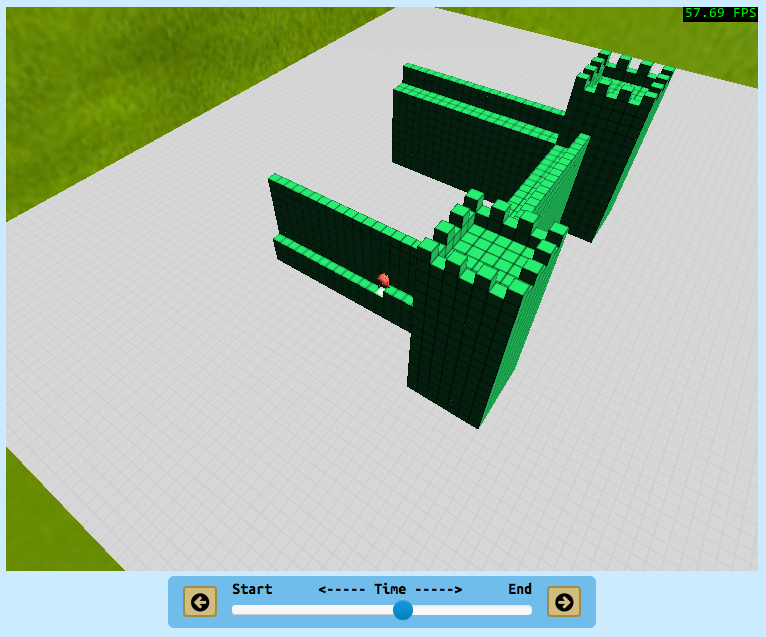
\includegraphics[width=0.9\columnwidth]{images/castle-time-slider}
  \caption{A screenshot of the castle pogram in the middle of execution. The time slider (shown) can be used to scrub execution forward and backward. The resolution of the time slider is not as fine-grained as the total number of states, but the right/left buttons allow moving one state forward/backward, thus the user can jump to arbitrary states.}
  \label{fig:time-slider}
\end{figure}

\section{Technique} 

In addition to the existing, na\"{i}ve implementation, we implemented two new approaches to simulating program in \da. The goal for all of these techniques is to support jumping to arbitrary point in execution (where each command is one step) and getting the world state for that point. The original implementation did this by simply keeping a copy of the world state for every single command executed, which was very simple but scales very poorly for large programs. For the purposes of this project, ``large'' programs mean those with more than 100,000 commands. The example castle program in Appendix~\ref{app:castle-code} is almost 10,000 commands, for example.

\subsection{Checkpointed Simulation}
The first approach we implemented was mostly intended as a baseline for comparison. Instead of storing literally every state, this approach stores a set of \emph{checkpoint} states along with the simulation context for that state. In order to jump to an arbitrary state, the simulator starts executing from the nearest checkpoint before the desired state and runs the simulation as normal to that state. We expected this approach to see a speed-up approximately proportional to the ratio of number of checkpoints to total number of states, since the na\"{i}ve implementation's runtime was dominated by copying states.

\subsection{World Delta-Based Simulation}
Because we need to execute the program immediately, there is no benefit to doing static analysis. We instead do dynamic analysis. There is no input to the program, and therefore no non-determinism. Thus, we are in a sense trying to evaluate a very big constant expression.

\subsubsection{World State Detlas}

World state deltas consist of two components: (1) a delta on the position and direction of the dragon and (2) a delta on the cubes present in the world. Deltas are created from a sequence of commands, and are independent of a specific starting state. They simply represent the change to an arbitrary state that would result if that sequence of commands is applied. 

Taking the position delta first, a na\"{i}ve approach (and, indeed, our initial approach) would be to represent it as an absolute delta in terms of the x-, y-, and z-dimensions. This is incompatible, however, with the nature of our language. Our language does not have movement commands like \texttt{move in the x direction} that specify an absolute direction. Instead it has a \texttt{forward} command whose effect is relative to the dragon's current heading. 

This means a position delta must be represented such that it can be relative to any given initial direction. Our solution is to represent a position delta as a distance parallel to the initial direction, and a distance perpendicular to the initial direction. When it comes time to apply the position delta to a concrete state, this information is combined with the dragon's initial direction to generate the delta in absolute terms. This only accounts for the dragon's position in the x-z plane. The two other pieces of the dragon's state, its direction and y-position, are represented separately. 

Since the dragon can never be facing up or down, and moves in those directions with specific \texttt{up} and \texttt{down} commands, the change in y-position can be stored as an absolute delta. Change in the dragon's direction can also be represented as a single integer. When computing a delta, we increment a counter for every right turn and decrement that counter for every left turn. It is thus easy to compute the dragon's new direction when applying a delta.

The final wrinkle of position deltas is the restriction that the dragon cannot go below the ground ($y=0$). If it is told to go \texttt{down} when already at ground level, it simple stays where it is. The impact of this is that a delta can only be relied upon if it would not move the dragon below the ground at any point. Hence, we track the greatest lower extent for each delta and application of a delta is conditional on the dragon's current y-position being higher than this extent. 

The delta on cubes is represented as a map from position deltas (as described above, though without tracking change in direction, as it is not needed) to cubes that should be added or removed. Applying this delta consists of processing each entry in the map, using the current dragon position and direction to compute an absolute position from the position delta, and then adding or remove a cube at that location, as appropriate.

One critical assumption about the world state that allow this technique to work is that a delta can always be computed from only a list of commands; a concrete world state is not required. This only holds because our language does not support conditionals: any block of code will behave similarly regardless of the world state. They can be straightforwardly mapped to any concrete world state by transforming the delta relative to the dragon. We are planning on (eventually) implementing language features to allow conditions on, e.g., whether a block exists, so we will have to generalize this technique to support such a program. As a worst case, the system can at least fall back to a non-delta implementation for segments with conditions but use detlas elsewhere.

\subsection{Caching Procedures and Loops}

The only two constructs in the language for repetition are procedures and definite loops, and we primarily target these constructs for optimization. The overall goal is to compute a world state delta for each statement we wish to optimize. When we next see the same statement, rather than running the simulator, we try to apply the cached delta to our concrete world state. We call these procedures and loops \emph{cachable statements}.

We can only reuse cachable statements if they have the same concrete environment. In the language of \da{}, there are no global variables nor lexical closures for procedures. Therefore, the concrete parameters given to a procedure fully describe the environment. Likewise, for loops, we can fully describe the surrounding environment with the concrete values of the parameters passed to the procedure in which the loop is contained.

Optimized evaluation of a statement proceeds as follows. If the statement is not cacheable, we use the normal evaluation method. If it \emph{is} cachable, we first compute the surrounding concrete environment. This may involve evaluating the arguments passed to the procedure, or looking at the current set of in-scope variables. The environment and the pointer to the statement form a unique key. We use this key to look up a world delta from the cache. If one does not exist, we create the world delta for this statement by executing it normally. Note that this is recursive, so when computing a delta, we try to look up all subcommands in the cache. Thus, every concrete statement has its delta computed at most one time throughout execution. We then attempt to apply the world delta to the current world state. If it cannot be applied (because it would move the dragon below the ground), we revert to the normal evaluation method \emph{for the current statement only}. We continue optmized evaluation of all subsequent statements. 

The end result is a final world state, and a cache populated with deltas for every cachable statement. This cache can be used to quickly compute arbitrary states, as described in the next section.

\subsection{Jumping to Arbitrary Point of Execution}

A point of execution is defined by the number of previous commands (or, equivalently, program states). In other words, a point of execution is the $n$th program state for some $0<n\le N$ where $N$ is the total number of states in the program. When a world state delta is cached, we store the number of states the delta represents. Therefore, jumping to an arbitrary point of execution is a matter of determining the appropriate combination of deltas to apply before switching over to straight simulation. In particular, we proceed greedily from the top down. Starting with the top-level delta (i.e., the delta for the entire program) we check if the current delta would move us beyong the execution point we want. If not, we apply the delta and move on to the subsequent delta. If the current delta would move us too far (as will be certainly be the case for the top-level delta unless we are trying to get to the final state), we descend one level, and begin trying to apply the sub-deltas that constitute the too-large delta. If a delta cannot be applied, we similarly descend and try sub-deltas. In the limit, we fall back on simulating basic commands. 

\section{Evaluation}
To evaluate our optimizations, we compared their performance on a suite of benchmark programs to the performance of various unoptmized versions. For both convenience and completeness, we created the benchmark programs ourselves rather than use specific programs created by users of our system. To date, no group of students have used \da{} for much more than an hour, and so none have progressed to creating programs of the size and complexity needed to sufficienty evaluate our optimizations. The set of benchmarks we created are representative, however, of the types of things students often attempt to build, and the way in which students tend to try and enter very large numbers in every input. 

\todo{results}

\section{Conclusion}
jumping to arbitrary states is tricky
checkpointing is competitive on all but the largest programs, and is tremendously less complex

\section{Distribution of Work}
Regarding division of labor, we have been working collaboratively on Dragon Architect for 14 months. We each implemented several independent optimizations and test cases, and worked together to combine these optimizations into our final algorithm.

\bibliographystyle{plain}
\bibliography{501-final-report}

\appendix

\section{The Castle Program}
\label{app:castle-code}
\begin{verbatim}
define Line(x)
    repeat x times
        PlaceCube(1)
        Forward(1)

define Gate()
    repeat 3 times # gate wall thickness
        repeat 9 times # gate height
            Line(7)
            Forward(6) # gate width
            Line(7)
            Up(1)
            Right()
            Right()
            Forward(1)
        repeat 1 times # wall above gate height
            Layer()
        Right()
        Forward(1)
        Down(10) # gate wall height
        Left()
    Up(10) # gate wall height
    Left()
    Forward(1)
    Right()
    repeat 2 times # gate battlement height
        Layer()
    Down(12) # gate height + gate battlement height
    Right()
    Forward(4)
    Right()
    Forward(1)

define Wall()
    repeat 3 times # wall thickness
        repeat 10 times # wall height
            Layer()
        Right()
        Forward(1)
        Down(10) # wall height
        Left()
    Up(10) # wall height
    Left()
    Forward(1)
    Right()
    repeat 2 times # wall battlement height
        Layer()
    Down(12) # wall + battlement height
    Right()
    Forward(4)
    Right()
    Forward(1)

define Layer()
    Line(20)
    Up(1)
    Right()
    Right()
    Forward(1)

define Tower()
    repeat 15 times # tower height
        repeat 4 times
            Line(6)
            Right()
        Up(1)
    Down(1)
    Forward(1)
    Right()
    Forward(1)
    Roof()
    Up(1)
    Right()
    Forward(6) # tower size
    Right()
    Forward(1)
    Right()
    Battlement()
    Down(15) # tower height 

define Roof()
    repeat 5 times # tower size - 1
        Line(5)
        Left()
        Forward(1)
        Left()
        Forward(5) # tower size - 1
        Left()
        Left()

define Battlement()
    repeat 4 times
        repeat 3 times # tower size ÷ 2
            PlaceCube(1)
            Up(1)
            PlaceCube(1)
            Forward(1)
            Down(1)
            PlaceCube(1)
            Forward(1)
        Right()

repeat 3 times
    Wall()
    Tower()
    Right()
    Forward(26)
    Left()
    Left()
Gate()
Tower()
\end{verbatim}

\end{document}

